\documentclass[9pt]{beamer}

%%pacotes referentes ao Beamer
%\useoutertheme{split}
%\setbeamertemplate{navigation symbols}{}

%\usetheme{beamertheme}
%\usebeamercolor{beamer-color name}

%\usetheme{Boadilla}
%\usecolortheme{dove}

\usetheme{CambridgeUS}
\usecolortheme{beaver}

% \usetheme{pittsburgh}
% \usecolortheme{dolphin}
%\usecolortheme{dove}
%\usecolortheme{seahorse}

%\usetheme{Montpellier}

%number in figures an tables -- beamer
\setbeamertemplate{caption}[numbered]

%Colocar no description
%[leftmargin=!,labelwidth=\widthof{Turma A}]
	
%pacotes usuais do latex
\usepackage[portuguese]{babel}
\usepackage[utf8]{inputenc}
\usepackage{bm}
\usepackage{graphicx}
\usepackage{subfigure}
\usepackage[round]{natbib}
\usepackage{tikz}
\usetikzlibrary{shapes,arrows}
\usepackage{natbib}
\usepackage{times}
\usepackage{calc} %computes the length of a string
\usepackage{dsfont} %pacote para o 1 estilisado para indicadora
\usepackage{enumerate} %permite fazer uns enumerates diferentes
\usepackage[font=small,labelfont=bf]{caption} %permite colocar um segundo caption
\usepackage{booktabs} % comando \toprule, \midrule e \bottomrule
\usepackage{times} %times new roman font
\usepackage{multirow} %comando \multirow
\usepackage{setspace}
\usepackage{xcolor} %texto colorido
\usepackage{booktabs} %costumized tabs
\usepackage{tikz}
\usepackage{hyperref}

\usetikzlibrary{decorations.pathreplacing}

%código para alinhar a esquerda os itens no description
\defbeamertemplate{description item}{align left}{\insertdescriptionitem\hfill}
\defbeamertemplate{enumerate item}{align left}{\insertdescriptionitem\hfill}



%AMS packages
\usepackage{amsmath}
\usepackage{amsfonts}
\usepackage{amssymb}

%Não quebre linhas
\binoppenalty=\maxdimen
\relpenalty=\maxdimen

%Comandos criados por mim
\DeclareMathOperator*{\argmin}{arg\,min}

\DeclareMathOperator*{\argmax}{arg\,max}


\DeclareMathOperator{\espe}{E}

\DeclareMathOperator{\spann}{span}

\DeclareMathOperator{\cov}{Cov}

\DeclareMathOperator{\vari}{Var}

\definecolor{darkgreen}{RGB}{0,100,0}

\newcommand{\cc}[1]{\textcolor{darkgreen}{\bf #1}}


%Informações para o primeiro slide
\date{}
\title[Boas-vindas!]{Introdução ao Semestre Letivo Suplementar}
\author[Gilberto  e Carolina]{Gilberto Pereira Sassi\\ Cartolina Costa Mota Paraíba}
\institute[IME -- UFBA]{Universidade Federal da Bahia \\ Instituto de Matem\'{a}tica e Estat\'{i}stica\\ Departamento de Estat\'{i}stica }

\begin{document}
	
\tikzstyle{decision} = [diamond, draw, fill=blue!20, 
text width=4.5em, text badly centered, node distance=3cm, inner sep=0pt]
\tikzstyle{block} = [rectangle, draw, fill=blue!20, 
text width=5em, text centered, rounded corners, minimum height=4em]
\tikzstyle{line} = [draw, -latex]
\tikzstyle{cloud} = [draw, ellipse,fill=red!20, node distance=3cm,
minimum height=2em]
	
%Slide inicial
\begin{frame}{}
	\maketitle
\end{frame}

\section{Como vai funcionar?}

\begin{frame}{}


\textbf{Atividades assíncronas:}
\vfill

\textcolor{darkgreen}{\bf Sala de bate-papo}

Você pode conversar com quem estiver na sala naquele momento. Temos duas salas:


\begin{description}
	\item[Quer tc?] Sala de bate-papo para qualquer assunto;
	\item[Papo nerd!] Sala de bate-papo pra assuntos relacionados ao curso;
\end{description}
\vfill
	
\textcolor{darkgreen}{\bf Aula on-line na sala virtual}
	
Encontro com a presença de Gilberto e Carolina, Professores/moderados do curso.

\begin{itemize}
	\item Tiraremos dúvida e explicaremos conceitos.
	\item Tolerância de 15 minutos.
	\item As serão gravadas e ficarão disponíveis no MOODLE.
\end{itemize}  

\end{frame}

\begin{frame}{}

\textbf{Atividades assíncronas}
\vfill


Total de \textcolor{darkgreen}{\bf 3 pontos} na nota final.
\begin{description}
	\item[WikiStat] Recurso para construir coletivamente com um documento ou página com todos os conceitos e técnicas deste curso. \textcolor{darkgreen}{\bf Vale 0,6 pontos};
	\item[Glossário] Coleção definições, nomenclaturas, e jargões usados em Estatística. \textcolor{darkgreen}{\bf Vale 0,6 pontos};
	\item[Diário] \textit{Diário de bordo} em que o participante anota o que estudou e como estudou. \textcolor{darkgreen}{\bf  Vale 0,6 pontos};
	\item[Portfólio] É um resumo individual de tudo o que vocês aprendendo neste curso.\textcolor{darkgreen}{\bf Vale 0,6 pontos};
	\item[Fórum: tire aqui suas dúvidas!] Fórum para tirar dúvidas. \textcolor{darkgreen}{\bf Vale 0,6 pontos.}
\end{description}


\normalsize
\end{frame}

\section{Avaliação}

\begin{frame}{Avaliação}

\cc{Provas:}

\begin{itemize}
	\item Serão duas provas com duração de 168 horas. A prova será entregue pelo MOODLE;
	\vfill
	
	\item Primeira prova (P1) começa no dia \cc{20/10/2020};
	\vfill
	
	\item Segunda prova (P2) começa no dia \cc{15/12/2020};
	\vfill
	
	\item Nota final: $NF = \dfrac{P1 + P2}{2}$;
	\vfill
	
	\item Aprovação se $NF \geq 5$;
\end{itemize}
\vfill

\cc{Bônus de participação:} Total de 3 pontos. 
\begin{itemize}
	\item \cc{WikiStat - 0,6 pontos}
	\item \cc{Glośario - 0,6 pontos}
	\item \cc{Diário - 0,6 pontos}
	\item \cc{Portfólio - 0,6 pontos}
	\item \cc{Fórum: tire aqui suas dúvidas! - 0,6 pontos}
\end{itemize}
\end{frame}


\section{Muita calma nessa hora}

\begin{frame}{Don't panic!}

\begin{itemize}
	\item Não vamos cobrar a presença;
	\vfill
	
	\item Caso você não alcance 5 pontos, essa reprovação não vai aparecer no seu histórico escolar;
	\vfill
	
	\item Caso você não alcance 5 pontos, essa reprovação não vai afetar o seu CR;
	\vfill
	
	\item Relaxe, fique calmo e foque em aprender;
	\vfill
	
	\item O importante é participar (vale três pontos);
	\vfill
	
	\item Outro importante é fazer os exercícios das listas de exercícios (Exercícios das provas serão idênticos das listas);
	\vfill
	
	\item Caso não alcance a aprovação, lembre que você estar super preparado para o {\bf Métodos Estatísticos} quando o ensino presencial voltar;
\end{itemize}

\end{frame}

\section{MOODLE: mãos na massa!}

\begin{frame}{}

Bora ver como funciona as atividades síncronas assíncronas no MOODLE. 

Hoje vai ser isso: vamos ver como funciona o MOODLE e semana que vem começamos o curso propriamente.

\begin{figure}[!htbp]
	\centering
	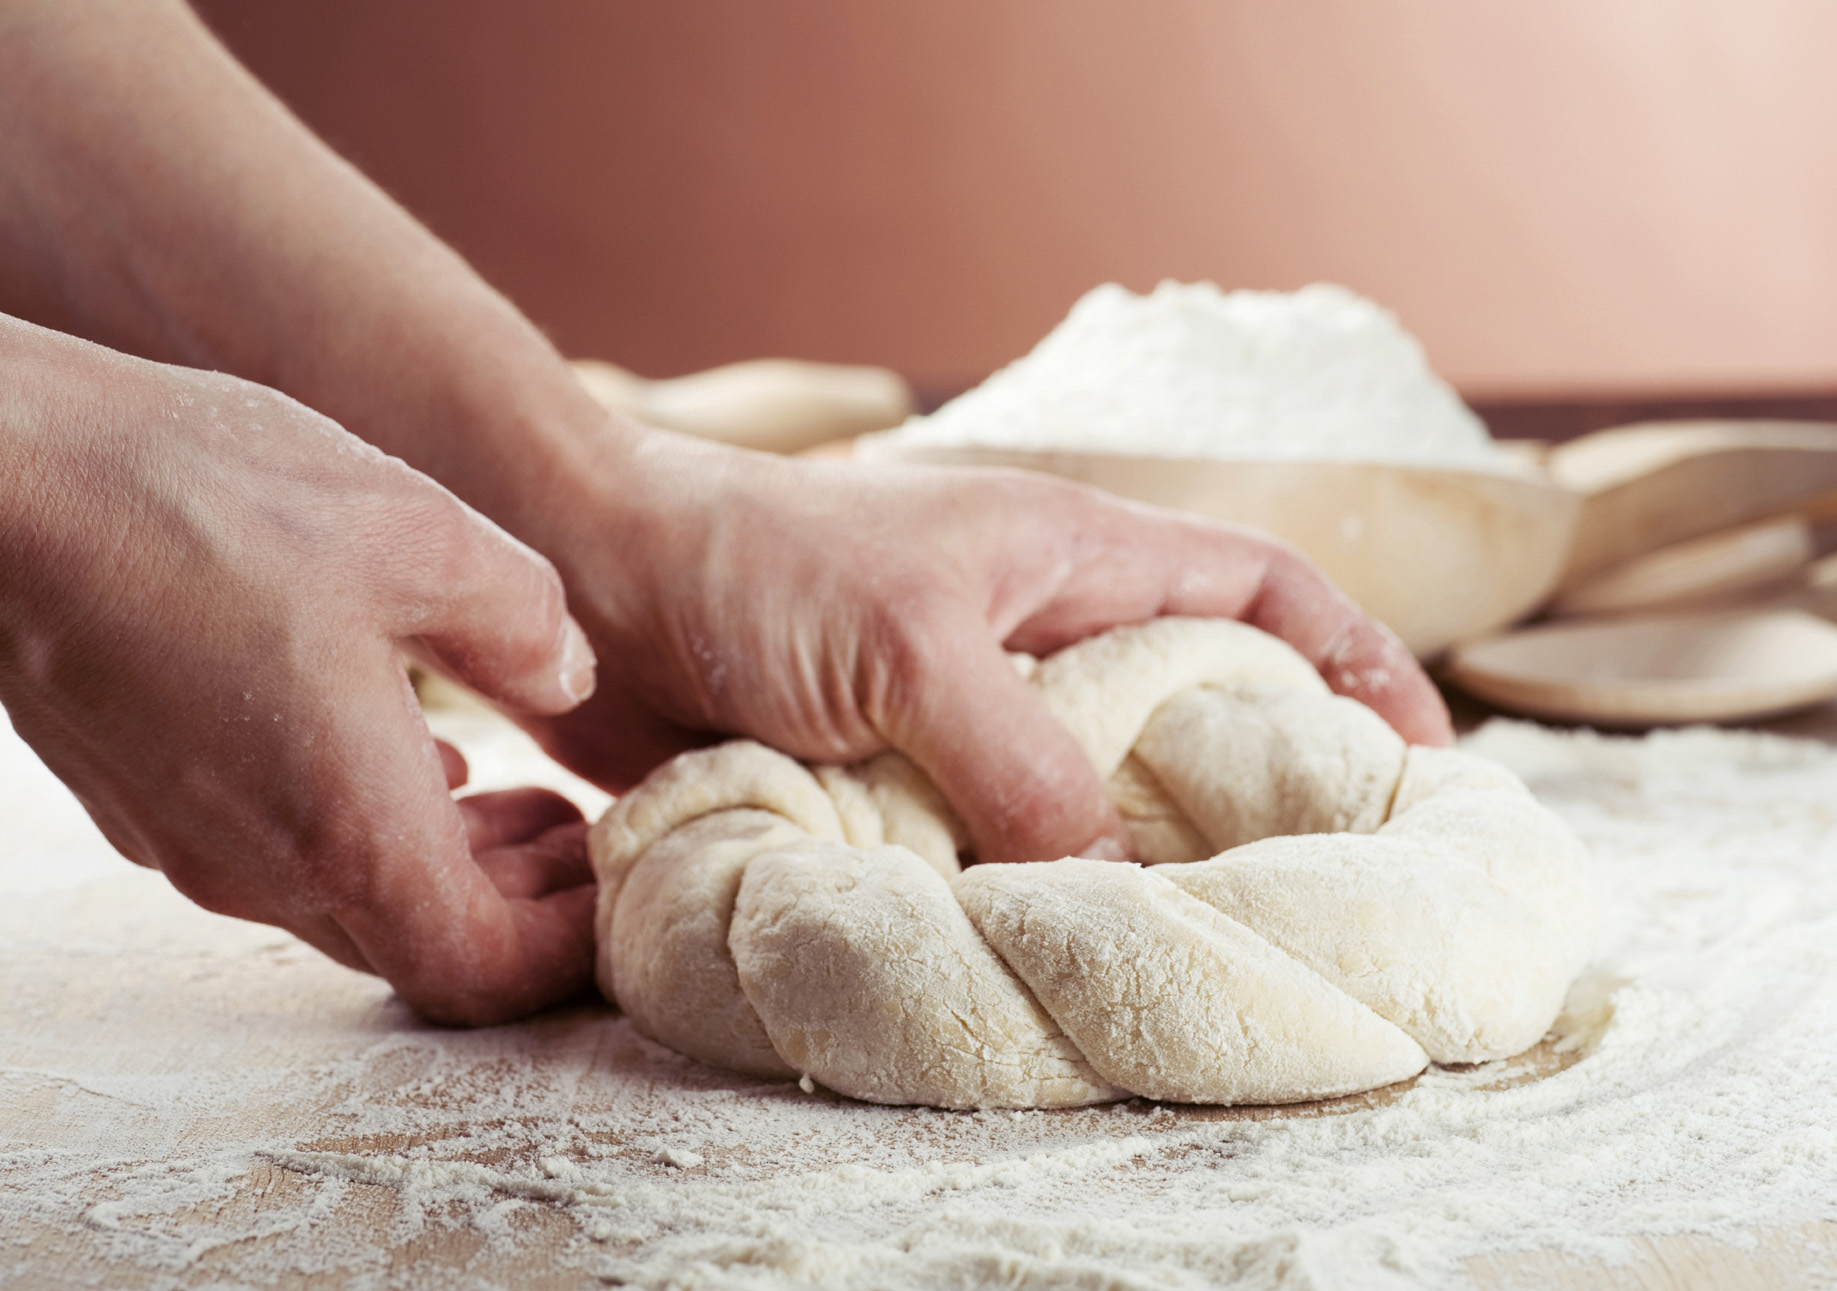
\includegraphics[width=0.75\linewidth]{oficina_de_macarrao_caseiro.jpg}
\end{figure}

\end{frame}

\end{document}